\section{Runtime Analysis}

To simplify the mathematical analysis, we assume that the input size is a power of two, i.e., $n = 2^p, p \in \mathbb{N}$.
We use the halving increment sequence defined previously with

\[
    h_i = \frac{n}{2^{t-i}}, 0 \leq i < t
\]

\noindent
Our focus lies on analyzing the number of calls for the labeled positions in Listing~\ref{lst:shell}: $c_1$, $c_2$, $c_3$.

For demonstration purposes, we choose $p=4$, and an array guaranteed to be sorted in strictly descending order (see Figure~\ref{fig:bestcase}).
Such a configuration contributes to a better understanding of the individual passes of the algorithm, which will be visually illustrated in the following.
\begin{figure}[!h]
    \centering
    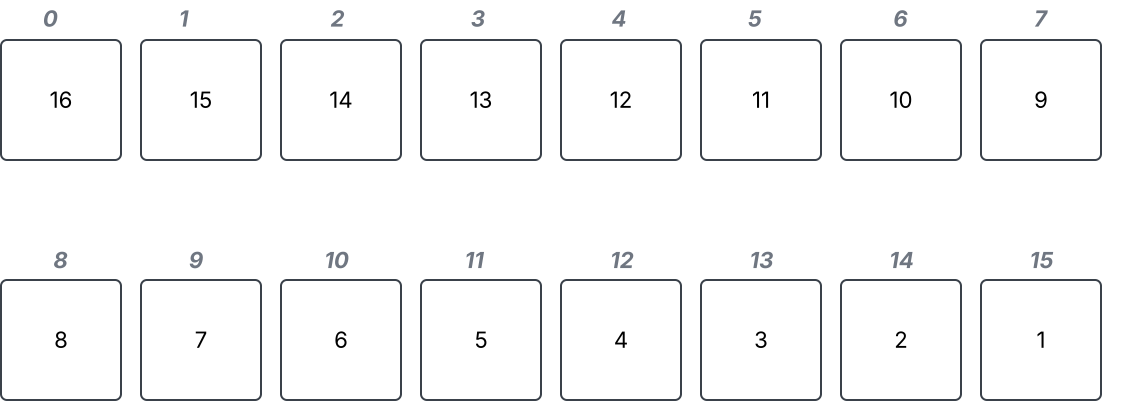
\includegraphics[width=1\columnwidth]{img/bestcase-sequence}
    \caption{A sequence of $16, \ldots, 1$ for demonstrating Shellsort-behavior on an unsorted array.}
    \label{fig:bestcase}
\end{figure}
Obviously, $c_1$ is called $\lg n$ times due to the halving sequence used in the algorithm (we ignore the loop condition in the following analysis, which would otherwise yield $\lg n + 1$ calls).
The starting value of \texttt{i} in each pass is the current value of \texttt{delta}\footnote{
For the example with $n = 16$, this results in the sequence $8, 4, 2, 1$.
}, and it runs up to $n - 1$.
Thus, each full iteration of the loop corresponds to $c_2$ being called

\[
(n - 1) - \texttt{delta} + 1 = n - \texttt{delta}
\]

\noindent
times.
Considering also the outer loop, $c_2$ computes to

\[
\sum_{i=1}^{\lg n} \left( n - \frac{n}{2^{i-1}} \right)
\]

\noindent
which simplifies to:

\[
n \cdot \lg n - n + 1
\]

\noindent
This evaluates to $16 \cdot \lg 16 - 16 + 1 = 49$ for our example.
Note that this derivation assumes $n = 2^p$ for some $p \in \mathbb{N}$.
For the general case, the total number of $c_2$ calls can be expressed as:

\[
    \sum_{i=1}^{\lfloor \lg n \rfloor} \left( n - \left\lfloor \frac{n}{2^i} \right\rfloor \right)
    = n \cdot \lg n - \sum_{i=1}^{\lfloor \lg n \rfloor} \left\lfloor \frac{n}{2^i} \right\rfloor
\]

\noindent
Table~\ref{tab:counts} shows the number of invocations for $c_2$ for various input sizes.
For $n > 2156$, the empirical count $c_2$ falls below $n^\frac{4}{3}$, while for $n \geq 982$, the inequality $n^\frac{4}{3} > n\ \lg\ n$ holds, as pointed out earlier.


\begin{table}[h!]
    \centering
    \begin{tabular}{r|r|r|r|r|r}

        \textbf{$n$} & \textbf{$c_2$} & \textbf{$n^{1.1}$} & \textbf{$n^{\frac{4}{3}}$} & \textbf{$n \log n$} & \textbf{$n^2$} \\
        \hline
        8     & 17     & 10     & 16     & 24     & 64      \\
        16    & 49     & 21     & 40     & 64     & 256     \\
        32    & 129    & 45     & 102    & 160    & 1024    \\
        64    & 321    & 97     & 256    & 384    & 4096    \\
        128   & 769    & 208    & 645    & 896    & 16384   \\
        256   & 1793   & 455    & 1620   & 2048   & 65536   \\
        1024  & 9217   & 2094   & 10240  & 10240  & 1048576 \\
        2156  & 21565  & 4592   & 23328  & 23867  & 4648336 \\
        2157  & 21576  & 4597   & 23344  & 23884  & 4652649 \\
        2158  & 21586  & 4600   & 23360  & 23901  & 4656964 \\
        \ldots & \ldots & \ldots & \ldots & \ldots & \ldots \\
        10000 & 120005 & 25118  & 158489 & 132877 & 100000000 \\
        100000 & 1500006 & 316227 & 3162280 & 1660964 & 10000000000 \\
        200000 & 3200006 & 677850 & 7786440 & 3521928 & 40000000000 \\
        500000 & 8500007 & 1857235 & 25600000 & 9465784 & 250000000000 \\
        1000000 & 18000007 & 3981072 & 63000000 & 19931568 & 1000000000000 \\
        \hline
    \end{tabular}
    \smallskip
    \caption{Comparison of $c_2$ counts against bounds for vaious $n$.}
    \label{tab:counts}
\end{table}

While $c_2$ reflects only one level of the outer loop, $c_3$ is expected to dominate and contribute significantly to the algorithm's complexity toward the upper bound of $O(n^2)$. $c_3$ is representing the innermost \texttt{while}-loop: Here, the algorithm checks whether the elements $j$ and $j - \texttt{delta}$ need to be reordered.
If so, the elements at these positions are swapped until the current $h_i$-sequence is locally sorted.
As a result, the array becomes relatively sorted with respect to the pairs of elements that are $h_i$ positions apart.
For our example with $n = 16$ and $h_3$, the following relative pairings are created:

\begin{itemize}
    \item $(R_0, R_8)$
    \item $(R_1, R_9)$
    \item \ldots
    \item $(R_7, R_{15})$
\end{itemize}

\noindent
This behavior is illustrated with Figure~\ref{fig:bestcase-it1}.
With the given array initially sorted strictly descending, Shellsort produces two subsequences of length $8$, each sorted relatively to each other\footnote{
In the general case, however, Shellsort sorts \textbf{interleaved} $h$-subsequences. See \cite{Knu97b} for examples.
}.

\begin{figure}[!h]
    \centering
    \includegraphics[width=1\columnwidth]{img/bestcase-it1}
    \caption{After the first pass, elements are relatively sorted within their respective $h_3$-spaced subsequences.}
    \label{fig:bestcase-it1}
\end{figure}
